\newpage

\section{Preparation} \label{preparation}
Before you start with the tutorial, it is important that the lab environment is configured. This section will guide you through the configuration. In this section, you will learn to install and configure the basics of:

\begin{itemize}
    \item Configure the \opnsense\ firewall using the VMware hypervisor.
    \item Create a virtual network in VMware.
    \item Install an extra network interface on the hypervisor that runs the \opnsense\ firewall.
\end{itemize}

\tipbox{There could be newer versions of the operating systems than being used in this tutorial. If another version is downloaded and used, it will in most cases, not impact the tutorial. If problems are encountered, change to the version used in this tutorial}

\subsection*{Prerequisites}
Make sure that you have installed VMWare before you start on this task. As a Noroff student, you can log in and download VMWare from \url{www.onthehub.com}. You should have received a link with information about this earlier. How to install VMWare is not included in this tutorial. VMWare has a tutorial that can be used: \url{https://kb.vmware.com/s/article/2053973}

\begin{importantblock}
\textbf{If you want to use a different client or virtual hypervisors, you are \Rtext{on your own}!}
\end{importantblock}

There is expected that you know how to create and deploy a virtual server, so the creation of the Ubuntu machines is not covered in this tutorial. The \opnsense\ firewall has some additional configurations that need to be done, so the installation and configuration are detailed.

\subsection{Ubuntu Desktop}
\dlblocknar{The latest version of Ubuntu Desktop can be found at: \url{https://ubuntu.com/download/desktop}.} The version that is used in this tutorial is \cmd{Ubuntu 20.04.2.0 LTS}

If you need any help during the process of installing the Ubuntu Desktop, find a tutorial online that you can use. For example; \url{https://linuxhint.com/install_ubuntu_vmware_workstation/}. Or you could ask one of your fellow students or ask on Teams.

\subsection{Ubuntu Server} \label{ubuntu_server}
\dlblocknar{The latest version of Ubuntu Server can be found at: \url{https://ubuntu.com/download/server}.} The version that is used in this tutorial is \cmd{Ubuntu Server 20.04.2 LTS}

If you need any help during the process of installing the Ubuntu Server, find a tutorial online that you can use. For example; \url{https://blog.eldernode.com/install-ubuntu-20-04-lts-server-on-vmware/}. Or you could ask one of your fellow students or ask on Teams. 

\subsection{\opnsense} \label{opnsense_setup}

\dlblocknar {Download \opnsense\ from \url{https://opnsense.org/download/}. Chose \Btext{amd64}\ architecture, \Btext{dvd}\ as the image type. The chosen location to download from does not matter, but normally a location that is close to your location is the fastest one when downloading.}

Start with downloading the file and follow the configuration below:

\setupblock{\begin{enumerate}
    \item Go to \url{https://opnsense.org/download/} and chose the different options. The download page should look something like figure \ref{opnsense:download} now. The checksum (hash) will be different than in the figure.
    \item Before clicking on \Btext{Download}\ button, make sure to make a note with the SHA256 hash.
    \item The file you are downloading has a name similar to this: \cmd{OPNsense-20.7-OpenSSL-dvd-amd64.iso.bz2}.
    \item Check if your file has the same SHA256 hash as the one provided to you on the download page. Depending on what OS you are using, there are multiple methods to find the SHA256 hash of the file. Examples for Linux and Windows below:
    \begin{itemize}
        \item Linux: \cmd{sha256sum <Your OPNsense iso file>}
        \item Windows: \cmd{certutil -hashfile <Your OPNsense iso file> SHA256}
    \end{itemize} 
    \item When the download is finished, extract the iso file from the compressed archive. You should now have a \cmd{.iso} file.
\end{enumerate}}

\tipbox{Using hashes to verify the authenticity of the file is important. Also, do this for the Ubunto iso files you downloaded.}

\begin{importantblock}
    Do not extract the .iso file. If it is extracted, it will not work properly.
\end{importantblock}

\begin{figure}[h!]
    \centering
    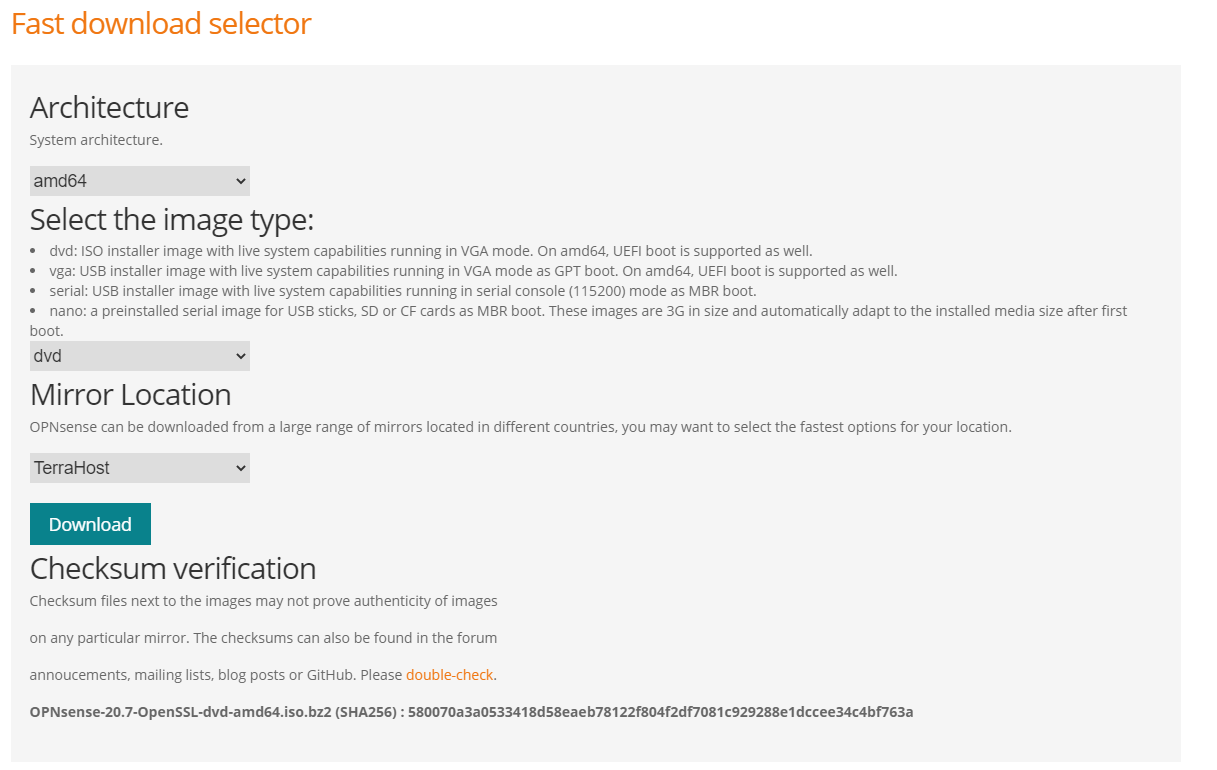
\includegraphics[width=0.7\textwidth]{Images/opnsense_download.PNG}
    \caption{An example of the download page for \opnsense}
    \label{opnsense:download}
\end{figure}

\quesblock{\begin{enumerate}
    \item[2.] What is a hash?
    \item[3.] Did your hash values match?
\end{enumerate}}

\subsection{Create a virtual network in VMware} \label{virt_network}
Now you can start to configure a virtual network in VMWare. This is important since all the clients we are creating must be in the same network.

\setupblock{\begin{enumerate}
    \item In VMWare go to \cmd{Edit} and click on \cmd{Virtual Network Editor}.
    \item Click on \cmd{Add Network}. Name it \textbf{VirtNetwork2}.
    \item Make sure it is a \cmd{Host-Only} network.
    \item Deselect this two options if they are selected:
    \begin{itemize}
        \item \cmd{Connect a host virtual adapter to this network}.
        \item \cmd{Use local DHCP service to distribute IP address to VMs}.
    \end{itemize}
    \item Set the IP you want and the subnet mask of 255.255.255.0 (CIDR \textbackslash 24). This is the subnet we are using as our LAN network later. It does not matter what you are using as IP here, but in this tutorial we are using 192.168.20.0. If you use a different IP, write it down in your notes.
    \item The result should look something like figure \ref{opnsense:vmware_virt_network} now. 
    \item Click \cmd{OK} to save.
\end{enumerate}}

\begin{figure}[h!]
    \centering
    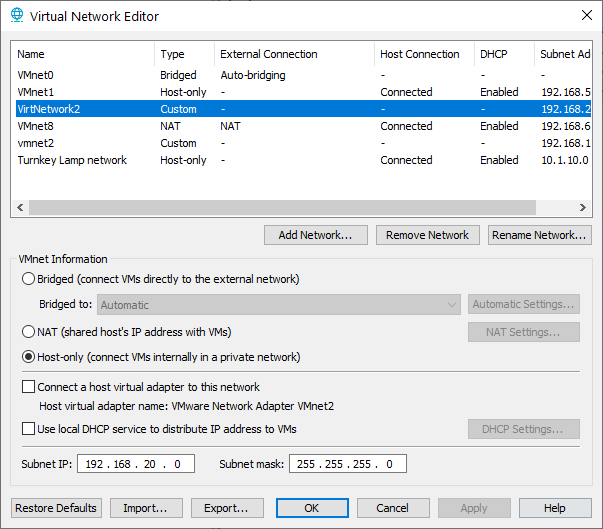
\includegraphics[width=0.6\textwidth]{Images/opensense_vmware_network.PNG}
    \caption{VMWare virtual network configuration}
    \label{opnsense:vmware_virt_network}
\end{figure}

\warnblock{Remember to add the two Ubuntu clients to the virtual network you have created here.}

\quesblock{\begin{enumerate}
    \item[4.] Why do you create a virtual network?
\end{enumerate}}

\subsection{The first configuration of the firewall}
The next step is to create your virtual machine. During the creation, you need to add another network interface to the firewall. This network interface will be your WAN interface later on:

\setupblock{\begin{enumerate}
    \item Start VMWare.
    \item Go to \cmd{File} and click on \cmd{New Virtual machine}. 
    \item Choose \cmd{Typical} and click \cmd{Next}.
    \item Chose \cmd{Installer disk image-file} (iso) and point to the \cmd{.iso} file you downloaded earlier. Click Next.
    \item Set a name for the virtual machine and chose where you want to store it. Recommend that you are using an SSD or faster storage for it. Click Next.
    \item The default values for storage capacity are OK for this tutorial. Click Next.
    \item Click on Customize Hardware, and do this:
    \item \begin{enumerate}
        \item Set memory to 1024 MB.
        \item Processors to 1.
        \item Set network adapter to your custom virtual network created earlier.
        \item Click on the \cmd{Add} button and add a new \cmd{Network Adapter}. Set this adapter to bridged. This will be your WAN connection later in this tutorial.
    \end{enumerate}
    \item Click \cmd{Close}, and \cmd{Finish}.
\end{enumerate}}

You are now ready to start your virtual firewall for the first time. Start your virtual machine with \opnsense.

\setupblock{\begin{enumerate}
    \item If the boot process was without errors, you should have heard a sound.
    \item Check that your \cmd{em0} is LAN and \cmd{em1} is WAN. At this moment, do not panic if your LAN IP is not correct, it will be fixed later.
    \item Use the username \cmd{installer} and the password \cmd{opnsense} to start the installing process.
    \item Accept all default values in the setup wizard. Leve root password blank, then it will be the password we provided when we logged in as installer.
    \item When asked for a reboot, do it.
    \item When the reboot is done, you will see that the LAN IP is 192.168.1.1. This is always the default IP for \opnsense.
    \item Now we are leaving the \opnsense\ virtual machine running, do not turn it \Rtext{off}.
    \item Start your Ubuntu Desktop and navigate to 192.168.1.1 using a browser. Like figure \ref{opnsense:opnsense_login}.
    \item Use the username and password you got, to log in. (the username: root and the password: opnsense)
    \item The setup wizard will start automatically.
\end{enumerate}}

\begin{figure}[h!]
    \centering
    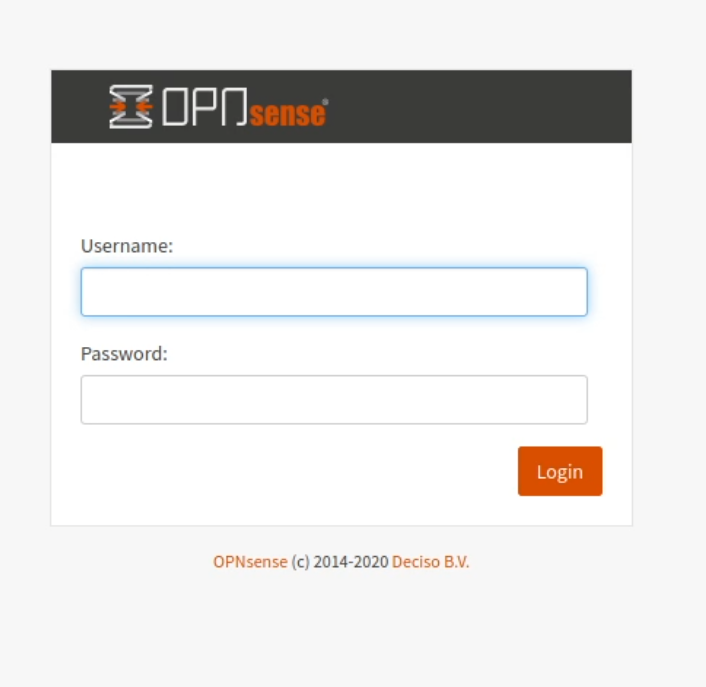
\includegraphics[width=0.5\textwidth]{Images/opnsense_login.PNG}
    \caption{\opnsense\ login screen}
    \label{opnsense:opnsense_login}
\end{figure}

Configuration using the wizard: \label{setup_wizard}

\setupblock{\begin{enumerate}
    \item Click \cmd{Next} when the wizard starts.
    \item Insert \cmd{Primary} and \cmd{Secondary} DNS servers. You can use the IPs for google's DNS. (8.8.8.8 and 8.8.4.4). Click \cmd{Next}. Read more about DNS in chapter \ref{DNSDHCP}.
    \item Set your \cmd{timezone}. Most likely to Europe/Oslo. Click \cmd{Next}.
    \item Remove the checkmark at RFC1918 Networks. Click \cmd{Next}.
    \item Change the LAN IP to \cmd{192.168.20.1}. (This will be your IP to \opnsense\ from your virtual network (LAN)). Click \cmd{Next}.
    \item Let the password be empty. (You then keep the password you created earlier). Click \cmd{Next}.
    \item Click \cmd{Reload}.
    \item Go to \cmd{192.168.20.1}, login, and you are welcomed with the dashboard of \opnsense.
\end{enumerate}}

\tipbox{If you have problems connecting to your \opnsense\ firewall via the browser after the reload, check your clients IP settings}

\quesblock{\begin{enumerate}
    \item[5.] What does the \cmd{em} in the network card stand for?
    \item[6.] Why did you remove the checkmark for RFC1918 Networks?
    \item[7.] Can you ping your firewall from your client? 
\end{enumerate}}

%\tipbox{There are multiple configurations in this tutorial, that require that a new virtual interface is made. If unsure on how to do it, check how it was done when you are configuring \opnsense\ with an extra interface in section \ref{opnsense_setup}.}

%\pline